\documentclass{article}
\usepackage[utf8]{inputenc}
\usepackage{amsmath}
\usepackage{systeme}
\usepackage{amssymb}
\usepackage[most]{tcolorbox}
\usepackage[scale=.95,type1]{cabin}
\usepackage{lmodern}

\usepackage[legalpaper,margin=1in]{geometry}

\setlength{\parindent}{10pt}
\setlength{\parskip}{1em}
\renewcommand{\baselinestretch}{1.2}

\title{Vector Spaces}
\date{}

\newcounter{example}[section]
\newenvironment{example}[1][]{\refstepcounter{example}\par\medskip
   \noindent \textbf{Example~\theexample. #1} \rmfamily}{\medskip}

\makeatletter
\renewcommand*\env@matrix[1][*\c@MaxMatrixCols c]{%
  \hskip -\arraycolsep
  \let\@ifnextchar\new@ifnextchar
  \array{#1}}
\makeatother

\newcommand\y{\cellcolor{blue!10}}
\newcommand\B{\textbf}
\newcommand\tcl{\begin{tcolorbox}[colback = {blue9}]}
\newcommand\etcl{\end{tcolorbox}}

\usepackage{tabularray}
\SetTblrInner{colsep=5pt,rowsep=1pt}

\newcommand\x{\times}

\makeatletter
\newcommand{\dashover}[2][\mathop]{#1{\mathpalette\df@over{{\dashfill}{#2}}}}
\newcommand{\fillover}[2][\mathop]{#1{\mathpalette\df@over{{\solidfill}{#2}}}}
\newcommand{\df@over}[2]{\df@@over#1#2}
\newcommand\df@@over[3]{%
  \vbox{
    \offinterlineskip
    \ialign{##\cr
      #2{#1}\cr
      \noalign{\kern1pt}
      $\m@th#1#3$\cr
    }
  }%
}
\newcommand{\dashfill}[1]{%
  \kern-.5pt
  \xleaders\hbox{\kern.5pt\vrule height.4pt width \dash@width{#1}\kern.5pt}\hfill
  \kern-.5pt
}
\newcommand{\dash@width}[1]{%
  \ifx#1\displaystyle
    2pt
  \else
    \ifx#1\textstyle
      1.5pt
    \else
      \ifx#1\scriptstyle
        1.25pt
      \else
        \ifx#1\scriptscriptstyle
          1pt
        \fi
      \fi
    \fi
  \fi
}
\newcommand{\solidfill}[1]{\leaders\hrule\hfill}
\makeatother

\begin{document}
    \section{Vectors in $\mathbb{R}^n$}
        
    A vector is characterized by 2 quantities: \textit{\B{length}} and \textit{\B{direction}}, and is represented by a directed line
    segment. But they are just 2 special types of vectors.

    \subsection{Vectors in the Plane}

    A \B{vector in the plane} is represented geometrically by a \B{directed line segment} whose \B{initial point}
    is the origin and whose \B{terminal point} is the point $(x_1, x_2)$. This vector is represented by the same 
    \B{ordered pair} used to represent its terminal point
    \[ \textbf{x} = (x_1, x_2)\]
    \begin{itemize}
        \item $x_1, x_2$ : the \B{components} of the vector \B{x}
        \item \B{u} $=$ \B{v} if and only if $u_1 = v_1$ and $u_2 = v_2$
    \end{itemize}

    \subsection{Vectors in $\mathbb{R}^n$}

    A vector in $n$-space is represented by an \B{ordered $n$-tuple}. The set of all $n$-tuple is called \B{$n$-space}
    and is denoted by $\mathbb{R}^n$.

    \tcl
    \B{Properties of Vectors Addition and Scalar Multiplication in $\mathbb{R}^n$}
    \begin{enumerate}
        \item \B{u} + \B{v} is a vector in $R^n$.
        \item \B{u}  + \B{v} = \B{v + u}
        \item \B{(u + v) + w = (u + (v + w))}
        \item \B{u + 0 = u}
        \item \B{u + (-u) = 0}
        \item $c$\B{u} is a vector in $R^n$.
        \item $c$\B{u + v} = c\B{u} + c\B{v}
        \item $(c + d)$\B{u} = $c$\B{u} + $d$\B{v}
        \item $c(d\B{u}) = (cd)\B{u}$
        \item $1(\B{u}) = \B{u}$
    \end{enumerate}
    \etcl

    \tcl
    \B{THEOREM 4.3 }\quad \textit{Properties of Additive Identity and Additive Inverse}
    \begin{enumerate}
        \item \B{v + u = v}, then \B{u =}$0$.
        \item \B{v + u = 0}, then \B{u = v}.
        \item 0v = 0 (scalar)
        \item c0 = 0 (vector $0$)
        \item cv = 0, then $c = 0$ or $v = 0$.
        \item $-(-v) = v$
    \end{enumerate}
    \etcl

    \subsubsection*{Writing a Vector as a Linear Combination of Other Vectors}

    Vector \B{x} can be written as the sum of scalar multiples of $n$ other vectors \B{$v_1, v_2, \cdots, v_n$}
    \[ x = c_1v_1 + c_2v_2 + \cdots + c_nv_n \]
    then the vector \B{x} is called a \B{linear combination} of the vectors \B{$v_1, v_2, \cdots, v_n$} 

    \section{Vector Spaces}
    
    \textit{Any} set that satisfies these aforementioned properties (or \B{axioms}) is called \B{vector space},
    and the objects in the set are called \B{vectors}.

    \B{Definition of Vector Space.} Let $V$ be a set on which 2 operations (\B{vector addtition} and 
    \B{scalar multiplication}) are defined. \B{u, v, w} $\in V$.\\
    $V$ is called a \B{vector space} if the listed axioms are satisfied for every \B{u, v, w} and
    real number $c, d$ :
    \tcl
    \begin{enumerate}
        \item 
            \B{u} + \B{v} in $V$
        \item \B{u}  + \B{v} = \B{v + u}
        \item \B{(u + v) + w = (u + (v + w))}
        \item \B{u + 0 = u} : $V$ has a \B{zero vector 0}
        \item \B{u + (-u) = 0} : For every \B{u} in $V$, there exists $-u$.
        \item $c$\B{u} in $V$
        \item $c$\B{u + v} = c\B{u} + c\B{v}
        \item $(c + d)$\B{u} = $c$\B{u} + $d$\B{v}
        \item $c(d\B{u}) = (cd)\B{u}$
        \item $1(\B{u}) = \B{u}$
    \end{enumerate}
    \etcl

    \B{REMARK.} A vector space consists of 4 entities:
    \begin{enumerate}
        \item a set of vectors
        \item a set of scalars
        \item 2 operations
    \end{enumerate}
    
    \B{Example 3.} \\
    1. The set of all $2 \x 3$ matrices with the operations of matrix addtition and
    scalar multiplication is a vector space.\\
    2. The set of all $2 \x 2$ matrices of the form $ \begin{bmatrix}
        a & b\\
        b & c
    \end{bmatrix}$ with the operations of matrix addition and scalar multiplication
    is a vector space.
    
    \B{Example. The Vector Space of All Polynomials of Degree 2 or Less} 

    Let $P_2$ be the set of all polynomials of the form 
    \[ p(x) = a_2x^2 + a_1x + a_0 \]
    with the usual operations of polynomial addition and scalar multiplication. $P_2$ is a 
    vector space. This can be extended to $P_n$.

    \tcl
        \B{Summary of Important Vector Spaces.}
        \begin{equation*}
            \begin{split}
                R & = \text{set of all real numbers} \\
                R^2 & = \text{set of all ordered pairs} \\
                R^3 & = \text{set of all ordered triples} \\
                R^n & = \text{set of all n-tuples} \\
                C(-\infty, \infty) & = \text{set of all continuous functions defined on the real number line} \\
                C[a, b] & = \text{set of all continuous functions defined on a closed interval} [a,b] \\
                P & = \text{set of all polynomials}\\
                P_n & = \text{set of all polynomials of degree} \le n \\
                M_{m,n} & = \text{set of all } m \x n \text{matrices} \\
                M_{n,n} & = \text{set of all square matrices}
            \end{split}
        \end{equation*}
    \etcl 

    \tcl
    \B{THEOREM 4.4 } \quad \textit{Properties of Scalar Multiplication}
    \[\begin{array}{ll}
        \text{1. } 0\B{v} = \B{0} & \text{2. } c\B{0} = \B{0} \\
        \text{3. If }c\B{v} = \B{0}, \text{then } c = 0 \quad   \text{or \B{v = 0}} & \text{4. } (-1)\B{v} = -\textbf{v}
    \end{array}\]
    \etcl

    \B{Example. } \\
    The Set of Integer is Not a Vector Space.\\
    The Set of Second-Degree Polynomials Is Not a Vector Space.
    \[ p(x) = x^2, \quad q(x) = -x^2 + x + 1 \implies p(x) + q(x) \notin V \]

    \section{Subspaces of Vector Spaces}

    \tcl
    \B{Definition of Subspace of a Vector Space.} \\
    A non-empty subset $W$ of a vector space $V$ is called a \B{subspace} of $V$ if $W$ is a vector space
    under the operations of addition and scalar multiplication defined in $V$.
    \etcl
    \B{Example 1.} The set $W = {(x_1, 0, x_3): x_1 \text{  and }x_3 \in \mathbb{R}}$ is a subspace of $\mathbb{R}^e$ with the
    standard operations. Graphically, it's the $xz$-plane.
    \begin{tcolorbox}
    \B{Test for a subspace.} If $W$ is a non-empty subset of $V$, then $W$ is a subspace of $V$ if and
    only if
    \begin{enumerate}
        \item $\B{u} + \B{v} \in W$
        \item $c\B{u} \in W$
    \end{enumerate}
    \etcl

    The 2 trivial subspaces are the \B{zero subspace} (contain only the zero vector), and the 
    space itself. The subspaces other than those 2 are \B{proper} (or nontrivial) subspaces.\\
    \B{Example. } The Set of Singular Matrices Is Not a Subspace of $M_{n,n}$.

    To prove, we need to show that $W$ is empty, $W$ is not closed under addtion, or $W$ is not closed
    under scalar multiplication. For this particular set, $W$ is not closed under addtion
    \[ A = \begin{bmatrix}
        1 & 0 \\ 0 & 0
    \end{bmatrix} , \quad B = \begin{bmatrix}
        0 & 0 \\ 0 & 1
    \end{bmatrix} \implies A + B \notin W\]

    \B{Note. } Sequences of subspaces nested within each other 
    \[P_o \subset P_1 \subset \cdots \subset P_n \]
    \B{Example 5. Subspaces of Functions (Calculus)}

    Let $W_5$ be the \textit{vector space} of all functions defined n $[0, 1]$, and let 
    \begin{itemize}
        \item $W_1 =$ set of all polynominal functions defined on the interval $[0,1]$
        \item $W_2 =$ set of all functions that are differentable on $[0,1]$
        \item $W_3 =$ set of all functions that are continuous on $[0,1]$
        \item $W_4 =$ set of all functions that are integrable on $[0,1]$
    \end{itemize}
    Show that $W_1 \subset W_2 \subset \cdots \subset W_5$, and $W_i \subset W_j$ for $i \le j$.
    \begin{center}
        \includegraphics*[width = 9cm]{images/Wcalculus.png}
    \end{center}

    \tcl
        \B{The Intersection of 2 Subspaces Is a Subspace. }
        If $V$ and $W$ are both subspaces of a vector space $U$, then $V \cap W$ is also a subspace of $U$.
    \etcl 
    \begin{center}
        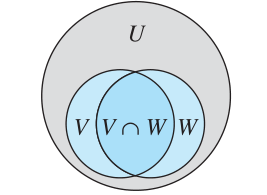
\includegraphics[width = 4cm]{images/VWintersection.png}
    \end{center}
    
    \subsection{Subspace of $\mathbb{R}^n$}
    
    \tcl
    \B{A characteristic of $\mathbb{R}^2$.} \quad If $W \subset R^2$, then it is a subspace if and only if
    \B{one} of the three possibilities listed below is true.
    \begin{enumerate}
        \item $W$ consists of the \textit{single point} $(0,0)$.
        \item $W$ consists of all points on a \textit{line} that pass through the origin.
        \item $W$ consists of all of $R^4$.
    \end{enumerate}
    \etcl 
    \begin{center}
        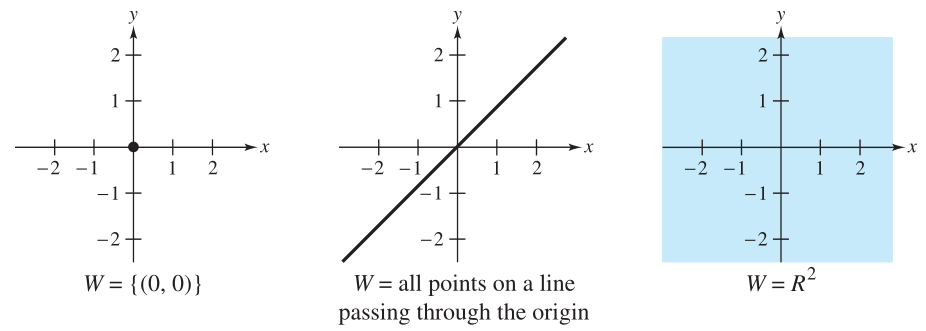
\includegraphics[width = 11cm]{images/3r2.png}
    \end{center}
    \B{Example 7.} The Set of all points on the circle $x^2 + y^2 = 1$ is not a subspace.\\
    \quad Take the sum $a = (0,1)$ and $b(1,0)$, then the Set is not closed under addtion.

    \B{REMARK. } Another way: a subspace of $\mathbb{R}^2$ must contain $(0,0)$.

    \subsection{Subspaces of $\mathbb{R}^3$}

    \tcl
    \B{Subspaces of $\mathbb{R}^3$. } $W \subset \mathbb{R}^3$ is a subspace of $\mathbb{R}^3$ (with the standard operations) if
    and only if it has \B{one} of the forms listed below.
    \begin{enumerate}
        \item $W$ consists of the \textit{single point} $(0,0)$.
        \item $W$ consists of all points on a \textit{line} that pass through the origin.
        \item $W$ consists of all points on a \textit{plane} that pass through the origin.
        \item $W$ consists of all of $R^3$.
    \end{enumerate}
    \etcl 

    \section{Spanning Sets and Linear Independence}

    \tcl
    \B{Def. Linear Combination of Vectors.} 

    A vector \B{v} in a vector space $V$ is called a \B{linear combination} of the vectors
    $\B{u}_1, \B{u}_2, \dots, \B{u}_k$ in $V$ if \B{v} can be written in the form
    \[ \B{v} = c_1\B{u}_1 + c_2\B{u}_2 + \dots + c_k\B{u}_k,\]
    where $c_1, c_2, \dots, c_k$ are scalars.
    \etcl 

    \B{Example 1. } 

    (a) For the set of vectors in $R^3$, 
    \[ S = {\overbrace{(1, 3, 1)}^{v_1}, 
        \overbrace{(0, 1, 2)}^{v_2},
        \overbrace{(1, 0, -5)}^{v_3}}, \]
   \quad  $\B{v}_1$ is a \B{linear combination} of $\B{v}_2$ and $\B{v}_3$ since $\B{v}_1 = 3\B{v}_2 + \B{v}_3$.

   (b) For the set of vectors in $M_{2,2}$, (page 226)

   \subsection{Finding a Linear Combination}
    \tcl
        \B{Def. Spanning Set of a Vector Space.} 

        Let $S = {\B{v}_1, \B{v}_2, \dots, \B{v}_k} \in V$. $S$ is called a \B{spanning set} of $V$ 
        if \textit{every} vector in $V$ can be written as a linear 
        combination of vectors in $S$. ($S$ \B{spans} $V$)
    \etcl 

    \B{Example.} $S = {(1,0,0), (0,1,0), (0,0,1)}$ spans $\mathbb{R}^3$ because any vector 
    \B{u} $= (u_1, u_2, u_3)$ can be written as 
    \[ \B{u} = u_1(1,0,0) + u_2(0,1,0) + u_3(0,0,1)\]

    \B{Example.} $S = {1, x, x^2}$ spans $P_2$ because any polynominal function
    $p(x) = a + bx + cx^2$ in $P_2$ can be written as
    \[p(x) = a(1) + b(x) + c(x^2) \]

    These above 2 spanning sets are called \B{standard spanning sets} of $R^3$ and $P_2$, respectively.

    \B{A nonstandard Spanning Set of $R^3$. }
    \[S_1 = {(1,2,3), (0,1,2), (-2,0,1)}\]
    \[ \systeme{
            c_1 - 2c_3 = u_1,
            2c_1 + c_2 = u_2,
            3c_1 + 2c_2 + c_3 = u_3
        } \]
    Since the coefficient matrix of the system has a nonzero determinant, this system has a unique solution.

    \B{A Set that Does Not Span $R^3$}
    \[ S_2 = {(1,2,3), (0,1,2), (-1,0,1)}\]
    \textit{does not} span $R^3$ since \B{w} $= (1, -2, 2)$ can not be expressed as a linear combination of these vectors.
    
    Consider these 2 aforementioned sets $S_1, S_2$. The vectors in $S_2$ lie in a common plane while those in $S_1$
    do not.
    \begin{center}
        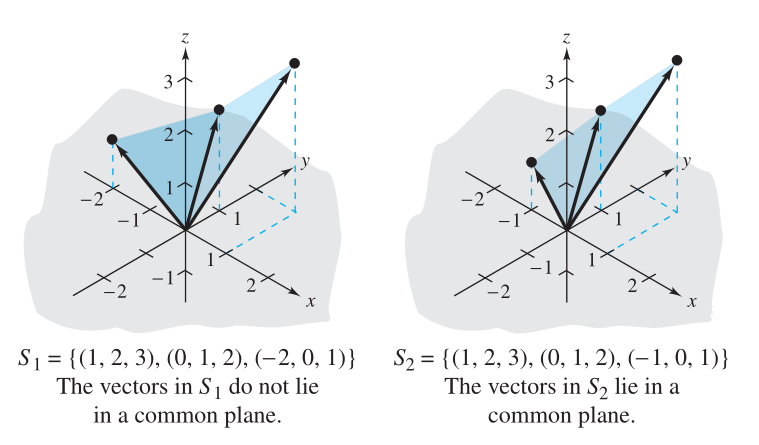
\includegraphics[width = 8cm]{images/S12span.png}
    \end{center}
    Although $S_2$ does not span $R^3$, it does span a subspace of $R^3$ - namely, the plane in which the 3 vectors of
    $S_2$ lie. This subspace is called the \B{span of $S_2$}.

    \tcl
        \B{Def. The Span of a Set.} 
        If $S = {\B{v}_1, \B{v}_2, \dots, \B{v}_k}$ is a set of vectors in $V$, then the \B{span of \textit{S}} is the set of
        all linear combinations of the vectors in $S$.
            \[ span(S) = span(v_1, v_2, \dots, v_k) = \{c_1v_1 + c_2v_2 + \cdots + c_kv_k : c_1, c_2, \dots, c_k \in \mathbb{R}\}\]
        If $span(S) = V$: $V$ is \B{spanned} by ${\B{v}_1, \B{v}_2, \dots, \B{v}_k}$, or $S$ \B{spans} $V$.
    \etcl 
    
    \tcl
    \textit{THEOREM 4.7} \quad \B{Span(S) Is a Subspace of $V$}

    If $S =$ $\{\B{v}_1, \B{v}_2, \dots, \B{v}_k\}$ is a set of vectors in $V$, then span($S$) is a subspace of $V$. Moreover,
    span($S$) is the smallest subspace of $V$ that contains $S$, in the sense that every other subspace of $V$ that
    contains $S$ must contain span($S$).
    \etcl 
    
%  $\{\B{v}_1, \B{v}_2, \dots, \B{v}_k\}$
% $ \{c_1v_1 + c_2v_2 + \cdots + c_kv_k $

    \subsection{Linear Dependence and Linear Independence}

    \tcl
    The set $S = $ $\{\B{v}_1, \B{v}_2, \dots, \B{v}_k\}$  in $V$ is called \B{linearly independent} if the
    vector equation 
    \[  c_1v_1 + c_2v_2 + \cdots + c_kv_k  = 0 \]
    has only the trivial solutions. If there are also nontrivial solutions, then $S$ is \B{linearly
    dependent}.    
    \etcl 
    
    \subsubsection{Testing for Linear Independence and Linear Dependence}
    \tcl
        Let $S = $ $\{\B{v}_1, \B{v}_2, \dots, \B{v}_k\}$ be a set of vectors n a vector space $V$. To determine 
        whether $S$ is linearly independent or not:
        \begin{enumerate}
            \item Write a homogeneous system of equations in the variables $c_1, c_2, \dots, c_k$
                \[\{c_1v_1 + c_2v_2 + \cdots + c_kv_k \]
            \item Determine whether the matrix of $k$ column vectors $v_1, v_2, \dots, v_k$ has a nonzero determinant
                or not.
            \item If yes, it is linearly independent. Otherwise, linearly dependent.
        \end{enumerate}
    \etcl 
    Example.(page 233)

    \tcl
    \textit{THEOREM 4.8 } \quad \B{A Property of Linearly Dependent Sets}
    A set $S$ containing $\ge 2$ vectors is linearly dependent if and only if at least 1 vector $v_j$ can be
    written as a linear combination of the other ones.
    \etcl


    If $S$ is linearly dependent, assuming $c_1 \ne 0$, then you can solve the equation for  $v_1$ and write
    $v_1$ as a linear combination of the remaining other ones. In other words, $v_1$ \textit{depends} on the other
    vectors on the set.
    \[v_1 = -\frac{c_2}{c_1}v_2 - \frac{c_3}{c_1}v_3 - \cdots - \frac{c_k}{c_1}v_k\]
    \B{Corolarry.} 2 vectors \B{u} and \B{v} in $V$ are linearly dependent if and only if one is a
    scalar multiple of the other.
    
    \section{Basis and Dimension}

    \tcl
    \B{Def. Basis}
    
        A set $S = \{\B{v}_1, \B{v}_2, \dots, \B{v}_n\}$ in $V$ is called a \B{basis} for $V$ if
        \begin{enumerate}
            \item $S$ spans $V$.
            \item $S$ is linearly independent.
        \end{enumerate}
    \etcl 
    \B{REMARK. } A basis has 2 features. It must have \textit{enough vectors} to span $V$, but \textit{not
    so many vectors} that 1 one them could even be written as a linear combination of the
    others in $S$.

    If $V$ has a basis consisting of a finite number of vectors, then $V$ is \B{finite dimesional}.
    Otherwise, like the vector space $P$ of all polynominals, is \B{infinite dimesional}.

    \B{Example 1. The Standard Basis for $\mathbb{R}^3$} 
    \[ S = \{ (1, 0, 0), (0, 1, 0), (0, 0, 1) \} \]
    \begin{itemize}
        \item $S$ span $\mathbb{R}^3$.
        \item $S$ is linear independent because the vector equation $c_1(1,0,0) + c_2(0,1,0) + c_3(0,0,1) = 0 $ 
            has only the trivial solution. Thus, $S$ is a basis for $\mathbb{R}^3$. 
    \end{itemize}
    That basis is called the \B{standard basis} for $\mathbb{R}^3$.  That is, the vectors
    \begin{equation*}
        \begin{split}
            \B{e}_1 & = (1,0,\dots,0)\\
            \B{e}_2 & = (0,1,\dots,0)\\
                    &\vdots\\
            \B{e}_n & = (0,0,\dots,1)
        \end{split}
    \end{equation*}
    form the \B{standard basis} for $\mathbb{R}^n$.

    \B{Standard Basis for $P_n$. } $S = \{1, x, x^2, \dots, x^n\}$

    \B{Standart Basis for $M_{2,2}$.} $S = \left\{\begin{bmatrix}
            1  & 0 \\ 0 & 1
    \end{bmatrix}, \begin{bmatrix}
            0 & 1 \\ 0 & 0
    \end{bmatrix}, \begin{bmatrix}
            0 & 0 \\ 1 & 0
    \end{bmatrix}, \begin{bmatrix}
            0 & 0 \\ 0 & 1
    \end{bmatrix}
    \right\}$

    \tcl
    \textit{THEOREM 4.9} \quad \textbf{Uniqueness of Basis Representation}
        If $S$ is a basis for $V$, \textit{every} vectors in $V$ can be written in \textbf{only one} way as a linear
        combination of vectors of $S$.
    \etcl 

    Now, these are 2 important theorems concerning bases.
    \tcl
    \textit{THEOREM 4.10} \quad \B{Bases and Linear Dependence}

    If $S$ is a set of $n$ vectors and is a basis for $V$, then every set contaning $\ge n$ vectors in $V$
    is \B{linearly dependent}.
    
    \textit{THEOREM 4.11} \quad \textbf{Number of Vectors in a Basis}
    If $V$ has one basis with $n$ vectors, then every basis for $V$ has $n$ vectors.

    \etcl 
    
    \subsection{The Dimension of a Vector Space}

    \tcl
        \B{Def. Dimension of a Vector Space.} 

        If $V$ has a basis with $n$ vectors, then $n$ is the 
        \B{dimension} of $V$, denoted by dim($V$) = $n$.
    \etcl
    If $V = \{ 0 \}$, dim($V$) $= 0$.
    \begin{enumerate}
        \item dim($R^n$) = $n$.
        \item dim($P_n$) = $n + 1$.
        \item dim($M_{m,n}$) = $mn$.
    \end{enumerate}
    If $W$ is $V$'s subspace, $W$ is finite dimensional and dim($W$) $\le n$.

    Example. 247

    \tcl
    \B{Basis Tests in an \textit{n}-Dimensional Space. } Let $V$ be a vector space of dimension $n$.
    \begin{enumerate}
        \item If $S = \{\B{v}_1, \B{v}_2, \dots, \B{v}_n\}$ is a linearly independent set of vectors 
            in $V \implies S$ is a basis for $V$.
        \item If $S = \{\B{v}_1, \B{v}_2, \dots, \B{v}_n\}$ spans $V \implies S$ is a basis for $V$.
    \end{enumerate}
    \etcl 

    \section{Rank of a Matrix and System of Linear of Equations}

    \tcl
        \B{\textit{Def.}Row Space and Column Space of a Matrix.} \quad  Let $A$ be a $m \x n$ matrix.
        \begin{enumerate}
            \item The \B{row space} of $A$  is the subspace of $R^n$ spanned by the \B{row vectors} of $A$.
            \item The \B{column space} of $A$ is the subspace of $R^m$ spanned by the \B{column vectors} of $A$.
        \end{enumerate}
    \etcl 
    Recall that 2 matrices are \B{row-equivalent} if one can be obtained from the other by elementary
    row operations.
    \tcl
    \textit{THEOREM 4.13} \quad \B{Row-Equivalent Matrices Have the Same Row Space.}

    If $A_{m\x n}$ is row-equivalent to $B_{m \x n}$, then they have the \textit{same} \B{row  space}.
    \etcl

    \B{REMARK. } The row space of a matrix does not change by elementary row operations. However, it can
    \textbf{change} the \textit{column space}.

    \tcl
    \B{Basis for the Row Space of a Matrix. } If $A$ is row-equivalent to a matrix $B$ in \textit{row-echelon} form, then the
    nonzero row vectors of $B$ form a basis for $A$'s \B{row space}.
    \etcl 

    Suppose you are ask to find a \B{basis} for the subspace spanned by $S = \{\B{v}_1, \B{v}_2, \dots, \B{v}_k\}$.

    \quad $\bullet$ Form a matrix $A$ consisting $B$'s vectors as \B{row vectors}. 

    \quad $\bullet$ Rewrite $A$ in \B{row-echelon} form.

    \textit{Find a Basis for the Column Space. } There are 2 options. On the one hand, the column space of $A$ is
    the row space of $A^T$. On the other hand, observe that:
    
    \B{REMARK.} Although row operations can \textit{change} the column
    space, they \textit{do not change} the \B{dependency relationships} between columns. \textit{(Notice that, the determinant 
    remains unchanged.)}

    \tcl
    \textit{THEOREM 4.15} $\quad$ \textbf{Row and Column Spaces Have Equal Dimension.}
    \etcl 
    \B{\textit{Proof.}} (p.256) Suppose the basis $S$ of $A$'s row space has $r$ vectors. You can rewrite the matrix and observe
    that the column vectors of $A$ are all linear combination of the vectors $S$. 

    Thus, dim(col space) $\le$ dim(row space). Doing the same, we have dim(row space) $\le$ dim(col space). Proof
    complete.

    \tcl
        \B{\textit{Def.} Rank of a Matrix. }
        The dimension of the row (or col) space of $A$ is called the \B{rank} of $A$, and denoted by rank($A$).
    \etcl 

    \subsection{The Nullspace of a Matrix}
    
    \tcl 
    \B{Solutions of a Homogeneous System. }

    Consider the homogeneous linear system $A_{m\x n}\B{x}_{n \x 1} = \B{0}$
    
    The set of all solutions of this is a subspace of $R^n$ called the \B{nullspace} :
    \[ N(A) = \{ \B{x} \in R^n : A\B{x} = \B{0}\} \]
    The dimension of $A$'s nullspace is the \B{nullity} of $A$.
    \etcl 
    \B{REMARK. } The \textit{nullspace} of $A$ is also the \B{solution space} of the system $A\B{x} = \B{0}$.

    \tcl 
    \B{Dimension of the Solution Space. }
    If $A$ is an $m \x n$ matrix of rank $r$, then the dimension of the nullspace is $n - r$. That is,
    \[ n = \text{rank}(A) + \text{nullity}(A) \]
    \etcl 

    Example. 261

    \subsection{Solutions of Systems of Linear Equations}

    The set of all solutions vectors of the \textit{homogeneous} linear system $A$\B{x} = \B{0} is a \B{subspace}.
    However, for $A\B{x} = \B{b} \ne 0$, it's not a subspace - since \B{0} is never a solution of a
    nonhomogeneous system. However, there is a \textit{relationship} between them.

    \tcl 
    \textit{THEOREM 4.18} \textbf{Solutions of a Nonhomogeneous Linear System.}

    If $\B{x}_p$ is a \textit{particular} solution for $A\B{x} = \B{b}$, then \textit{every} solution of this
    system can be written in the form
    \[ \B{x} = \B{x}_p + \B{x}_h \]
    where $\B{x}_h$ is a solution of $A\B{x} = \B{0}$.
    \etcl

    \B{Example 8. Finding the Solution Set of a Nonhomogeneous System.}

    Find the set of all solution vectors of the system of linear equations
    \[\systeme {
       x_1 - 2x_3 + x_4 = 5,
       3x_1 + x_2 - 5x_3 = 8,
       x_1 + 2x_2 - 5x_4 = -9
    }\]
    \textit{SOLUTION. } The augmented matrix for the system $A\B{x} = \B{b}$ reduces as follows.
    \[ \begin{bmatrix}[cccc|c]
        1 & 0 & -2 & 1 & 5\\
        3  & 1 & -5 & 0 & 8 \\
        1 & 2 & 0  & -5 & -9
    \end{bmatrix}   \rightarrow 
    \begin{bmatrix}[cccc|c]
        1 & 0 & -2 & 1 & 5 \\
        0 & 1 & 1 & -3 & -7 \\
        0 & 0 & 0 & 0 & 0
    \end{bmatrix} \]

    The system of linear equations corresponding to the reduced row-echelon matrix is 
    \[ \systeme {
            x_1 - 2x_3 + x_4 = 5,
            x_2 + x_3 - 3x_4 = -7
        } \]
    Letting $x_3 = s$ and $x_4 = t$, you can write a representative solution of $A\B{x} = \B{b}$ as follows.
    \begin{equation*}
        \begin{split} 
    \B{x} = \begin{bmatrix}
        x_1 \\ x_2 \\ x_3 \\ x_4 
    \end{bmatrix} = \begin{bmatrix}
        2s - t + 5 \\ -s + 3t - 7 \\ s + 0t + 0 \\ 0s + t + 0
        \end{bmatrix} & = s \begin{bmatrix}
        2 \\ -1 \\ 1 \\ 0
    \end{bmatrix} + t \begin{bmatrix}
    -1 \\ 3 \\ 0  \\ 1
    \end{bmatrix} + \begin{bmatrix}
        5 \\ -7 \\ 0 \\ 0 
    \end{bmatrix} \\
    & = s\B{u}_1 + t\B{u}_2 + \B{x}_p 
    \end{split}
    \end{equation*}

    \tcl
    \textit{THEOREM 4.19 } \textbf{Solutions of a System of Linear Equations}

    The system of linear equation $A\B{x} = \B{b}$ is consistent if and only if \B{b} is in the column
    space of $A$.
    \etcl 

    \subsection{Sys. Linear Equations with Square Coefficient Matrices}

    \tcl
    \textit{SUMMARY.} \B{Equivalent Conditions for Square Matrices.}

    If $A$ is an $n \x n$ matrix, then the following conditions are equivalent.
    \begin{enumerate}
        \item $A$ is invertible.
        \item $A\B{x} = \B{b}$ has a unique solution for \textit{any} $n \x 1$ matrix \B{b}.
        \item $A\B{x} = \B{0}$ has only the trivial solution.
        \item $A$ is row-equivalent to $I_n$.
        \item $det(A) = |A| \ne 0$
        \item Rank($A$) $= n$
        \item The $n$ row vectors of $A$ are linearly independent.
        \item The $n$ col vectors of $A$ are linearly independent.
    \end{enumerate}
    \etcl 

    \section{Coordinates and Change of Basis}

    If $B$ is a basis for $V$, then every vector \B{x} $\in V$ can be expressed in one and only one way as
    a linear combination of $B$'s vectors. The \textit{coefficients} in that linear combination are the \B{
        coordinates of x relative to B
    }. In the context of \textit{coordinate}, the order of vectors in basis is important, and this will
    be emphasized by referring to the basis $B$ as an \textit{ordered} basis.

    \tcl
    \textbf{Coordinate Representation Relative to a Basis.}

    Let $B = \{\B{v}_1, \B{v}_2, \dots, \B{v}_n\}$ be an \textit{ordered} basis for $V$, and let \B{x}$\in V$ such that
    \[ \B{x} = c_1\B{v}_1 + c_2v_2 + \cdots + c_nv_n \]
    The scalar $c_1, c_2, \dots, c_n$ are the \B{coordinates of x relative to the basis B}. The \textbf{coordinate
    matrix} (or \textbf{coordinate vector}) \textbf{of x relative to \textit{B}} is the column matrix in $\mathbb{R}^n$ whose components
    are the coordinates of \B{x}.
    \[ [\B{x}]_B = \begin{bmatrix}
        c_1 \\ c_2 \\ \vdots \\ c_n 
    \end{bmatrix} \]
    \etcl 

    \subsection*{Coordinate Representation in $\mathbb{R}^n$}
    
    Writing a vector in $R^n$ as \B{x}$ = (x_1, x_2, \dots, x_n)$ means that the $x_i$'s are the coordinates of \B{x}
    \textit{relative to the standard basis S} in $R^n$. So you have 
    \[ [\B{x}]_S = \begin{bmatrix}
        x_1 \\ x_2 \\ \vdots \\ x_n 
    \end{bmatrix} \]

    \B{Example. } The coordinate matrix of \B{x} in $R^2$ relative to the (nonstandard) ordered basis 
    $B = \{ \B{v}_1, \B{v}_2 \} = \{ (1,0), (1,2) \}$ is
    \[ [\B{x}_B] = \begin{bmatrix}
        3 \\ 2
    \end{bmatrix} \]
    Find the coordinate of \B{x} relative to the standard basis $B' = \{ \B{u}_1, \B{u}_2 \} = 
    \{ (1,0), (0,1) \} $.

    \textit{ANSWER. } $[\B{x}_B] = \begin{bmatrix}
        3 \\ 2
    \end{bmatrix}, \quad [\B{x}]_{B'} = \begin{bmatrix}
        5 \\ 4
    \end{bmatrix}$

    \begin{center}
        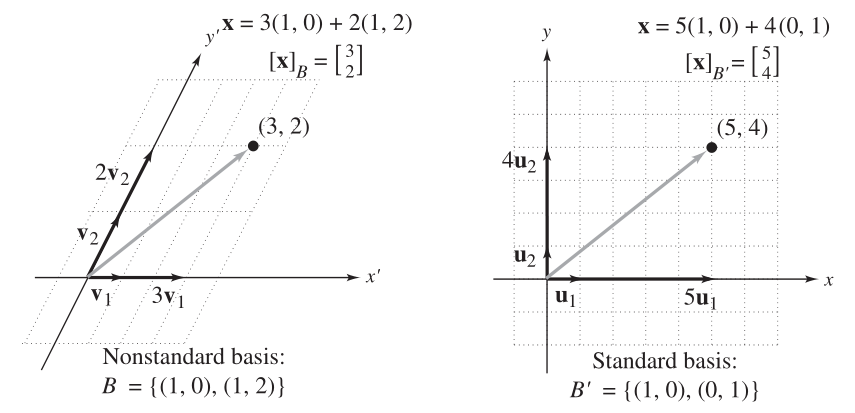
\includegraphics[width = 10cm]{images/2degplane.png}
    \end{center}

    \B{Example. } Find the coordinate matrix of \B{x} $= (1, 2, -1)$ in $R^3$ relative to the (nonstandard)
    basis 
    \[ B' = \{ \B(u)_1, \B{u}_2, \B{u}_3 \} = \{ (1,0,1), (0, -1, 2), (2, 3, -5)\} \]
    \textit{SOLUTION. } Begin by writing \B{x} as a linear combination of $\B{u}_1, \B{u}_2, \B{u}_3$ :
    \begin{equation*}
    \begin{split}
        \B{x} & = c_1\B{u}_1 + c_2 \B{u}_2 + c_3\B{u}_3 \\
        (1, 2, -1) & = c_1(1,0,1) + c_2(0,-1,2) + c_3(2,3,-5)
    \end{split}
    \end{equation*}
    Equating corresponding components produces the following system of linear equations
    \[ \systeme {
            c_1 + 2c_3 = 1,
            -c_2 + 3c_3 = 2,
            c_1 + 2c_2 - 5c_3 = -1
        } \]
        \[  \begin{bmatrix}
            1 & 0 & 2 \\ 
            0 & -1 & 3 \\
            1 & 3 & -5
        \end{bmatrix} 
        \begin{bmatrix}
            c_1 \\
            c_2 \\
            c_3
        \end{bmatrix} =
        \begin{bmatrix}
            1 \\
            2 \\
            -1
        \end{bmatrix} \]
    The solution of this system is $c_1 = 5, c_2 = -8, c_3 = -2$. So, the coordinate matrix of \B{x} 
    relative to $B'$ is 
    \[ [\B{x}_{B'}] = \begin{bmatrix}
        5 \\
        -8\\
        -2
    \end{bmatrix} \]

    \subsection{Change of Basis in $R^n$}

    In the previous example, 
    \begin{center}
        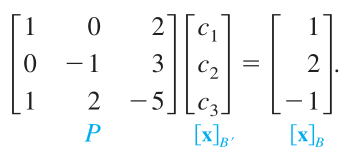
\includegraphics[width = 5cm]{images/P3.png}
    \end{center}

    The matrix $P$ is the \B{transition matrix from \textit{B'} to \textit{B}}.
    \[ P[\B{x}_{B'}] = []B{x}_B \]
    To perform a change of basis from $B$ to $B'$, use the matrix $P^{-1}$
    \[ [\B{x}_{B'}] = P^{-1}[\B{x}_B] \]
    This means that the change of basis problem in Eg.3 can be represented by the matrix equation
    \begin{center}
        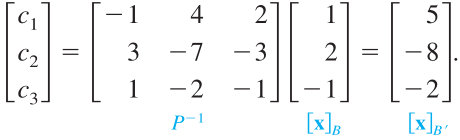
\includegraphics[width = 6cm]{images/P31.png}
    \end{center}

    \tcl
    \textit{THEOREM 4.20} \textbf{The Inverse of a Transition Matrix.}

    $P$ : \textit{transition matrix} from $B' \to B$ in $R^n$, then $P$ is \textbf{invertible} and $P^{-1}$ is the transition matrix 
    from $B \to B'$.
    \etcl

    \begin{tcolorbox}[colback = {red9}]
        \B{My own thoughts. } To perform a change of basis from $B$ to $S$, use $B$ itself 
        \[ B [\B{x}_B] = \B{x}_S \]
        Hence, for $[\B{x}]_B$ and $[\B{x}]_{B'}$ that is the same point
        \[ B[\B{x}_B] = B'[\B{x}_{B'}] = [\B{x}_S]\]
        To perform a change of basis from $B'$ to $B$, simply
        \[[\B{x}_B] = B^{-1}B'[\B{x}_{B'}]\]
        In other words, $P = B^{-1}B'$ (from $[\B{x}_{B'}] \to [\B{x}_B]$). And $P^{-1} = B'^{-1}B$ , we got a theorem.
    \end{tcolorbox}

    \tcl
        \textit{THEOREM 4.21} \textbf{Transition Matrix from \textit{B} to \textit{B'}.}  

        The matrix $P^{-1}$ from $B$ to $B^{-1}$ can be found by using Gauss-Jordan elimination on 
        \[ [B' \vdots B] \rightarrow [I_n \vdots P^{-1}] \]
    \end{tcolorbox}

    \subsection{Coordinate Representation in General $n$-Dimensional Spaces}

    \B{Example. } $p = 3x^3 - 2x^2 + 4$ has the coordinate matrix 
    $[p]_S = \begin{bmatrix}
        4 \\ 0 \\ -2 \\ 3
    \end{bmatrix}$.



    



\end{document}

